\documentclass[a4paper]{article}

\usepackage[english]{babel}
\usepackage[utf8]{inputenc}
\usepackage{amsmath}
\usepackage{graphicx}
\usepackage{caption}
%\usepackage{subcaption}
%\usepackage{float}
\usepackage{natbib}
\usepackage{floatrow}
\usepackage[label font=bf,labelformat=simple]{subfig}
\floatsetup[figure]{style=plain,subcapbesideposition=top}
\usepackage[margin=1.25in]{geometry}
\usepackage[table,xcdraw]{xcolor}
%\usepackage{lscape} use instead of below for printer friendly
\usepackage{pdflscape}
\renewcommand{\arraystretch}{2.5}
\usepackage[tableposition=top]{caption}

\renewcommand{\thepage}{S\arabic{page}}
\renewcommand{\thesection}{S\arabic{section}}
\renewcommand{\thetable}{S\arabic{table}}
\renewcommand{\thefigure}{S\arabic{figure}}
\captionsetup{labelfont=bf}


\title{Supplementary Figures for: Dysregulation of DNA Methylation in Human Intestinal Epithelial Organoids with Increasing Passage}

\author{Rachel Edgar}

\date{\today}

\begin{document}
\maketitle


\textbf{Table S1. Top over-represented GO groups in the list of genes adjacent to heteroskedastic CpGs.}Columns are: GO ID, name of the GO gene set, number of genes annotated to that gene set and associated to a heteroskedastic CpG, Benjamini-Hochberg corrected enrichment p value (which the data is sorted by), Multifunctionality (MF) score and the names of genes annotated to that gene set and associated to a heteroskedastic CpG.
\\
\\
\textbf{Table S2. Top over-represented GO groups in the list of genes adjacent to hypomethylated CpGs.} Columns are: GO ID, name of the GO gene set, number of genes annotated to that gene set and associated to a hypomethylated CpG, Benjamini-Hochberg corrected enrichment p value (which the data is sorted by), Multifunctionality (MF) score and the names of genes annotated to that gene set and associated to a hypomethylated CpG.
\\
\\
\textbf{Table S3. Top over-represented GO groups in the list of genes adjacent to hypermethylated CpGs.} Columns are: GO ID, name of the GO gene set, number of genes annotated to that gene set and associated to a hypermethylated CpG, Benjamini-Hochberg corrected enrichment p value (which the data is sorted by), Multifunctionality (MF) score and the names of genes annotated to that gene set and associated to a hypermethylated CpG.






\begin{figure}
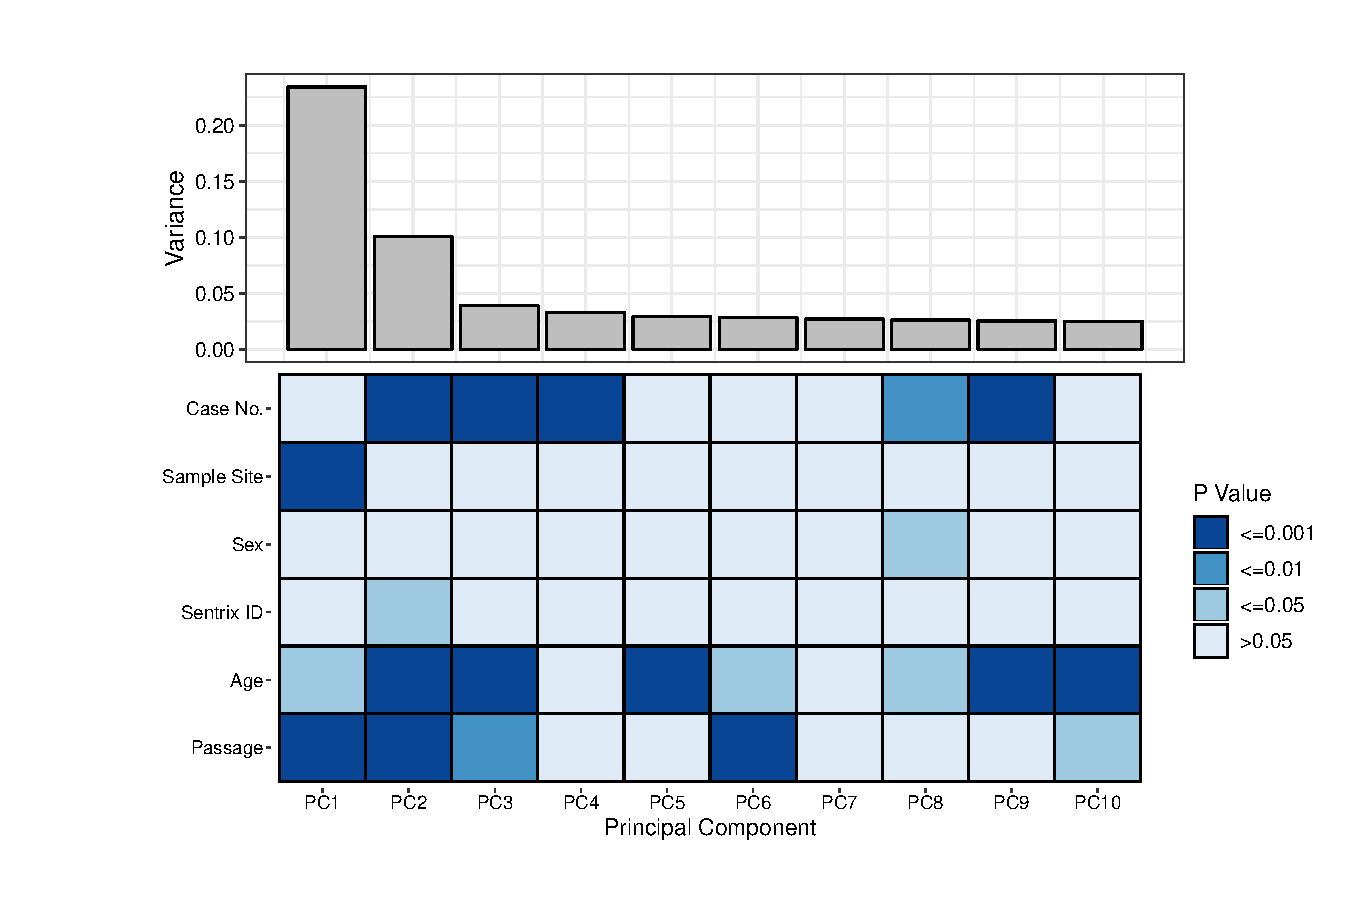
\includegraphics[width=1\textwidth]{../figs/heat_scree_EPIC_organoid.pdf}
\caption{\textbf{Sample site and passage contribute to the major components of variance in DNAm. } The scree plot shows the amount of DNAm variance accounted for by each PC. The heat map shows the associations between sample variables and each PC. P values were generated with a Spearman correlation for continuous variables or an ANOVA for categorical. }
\end{figure}

\begin{figure}
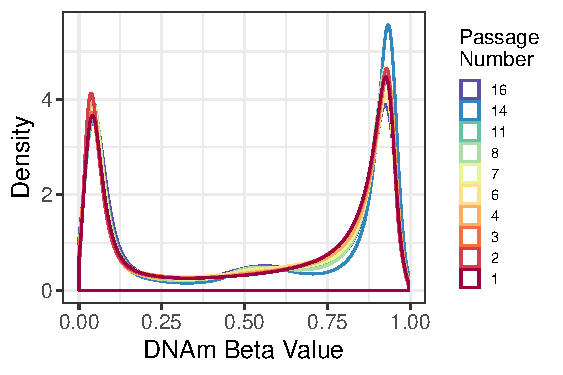
\includegraphics[width=0.90\textwidth]{../figs/Passage_all_CpGs.pdf}
\caption{\textbf{The DNAm beta value distribution for high passage samples is trimodial while for low passage samples it is bimodial.} All beta distributions displayed are for all  800,383 CpGs. (a) Beta value distributions for all samples at a given passage number. Curves are coloured by the passage number.}
\end{figure}

%\begin{figure}
%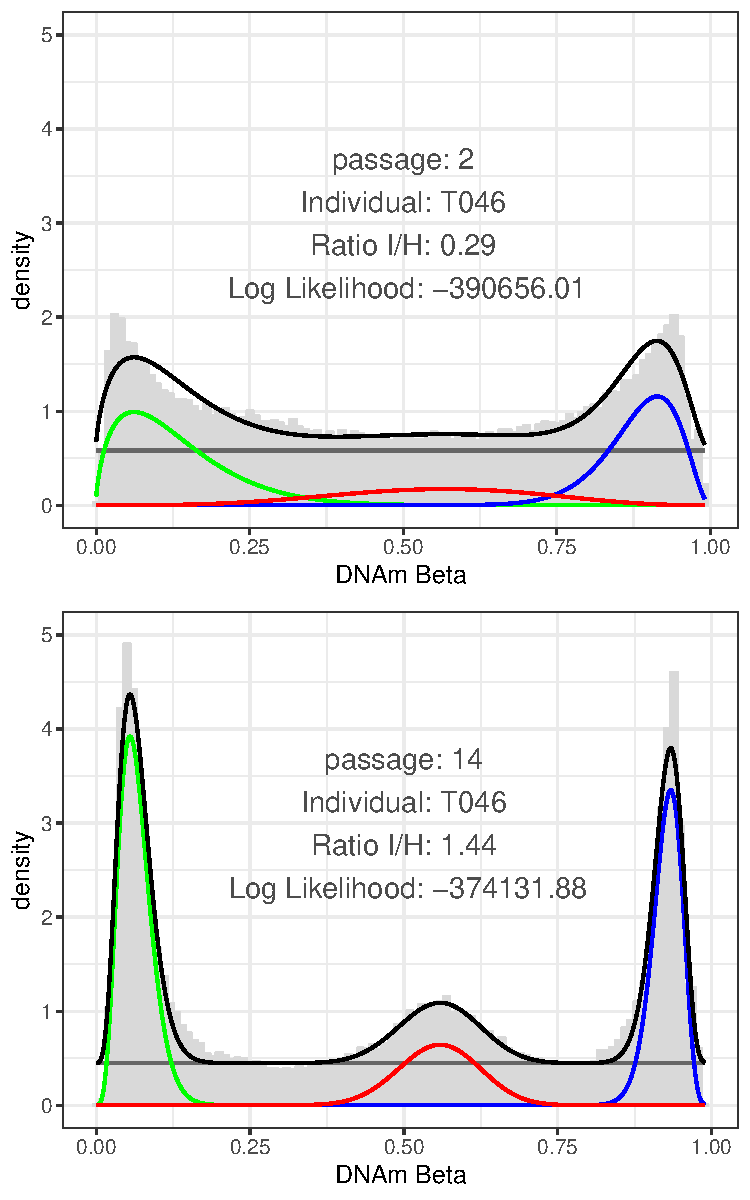
\includegraphics[width=0.6\textwidth]{../figs/Mix_model_Paired.pdf}
%\caption{\textbf{Fit of the mixture of beta-binomial distributions in two representative samples, one bimodal and one trimodal.} Both samples shown are from one individual which were passaged 2 and 14 times. The filled grey curve represents the actual beta value distribution, the coloured curves are the three beta-binomial distributions fit and the horizontal grey line represents the background uniform distribution fit. }
%\end{figure}





\begin{figure}
\begin{flushleft}

\begin{minipage}{.45\linewidth}
\sidesubfloat[]{\label{main:a}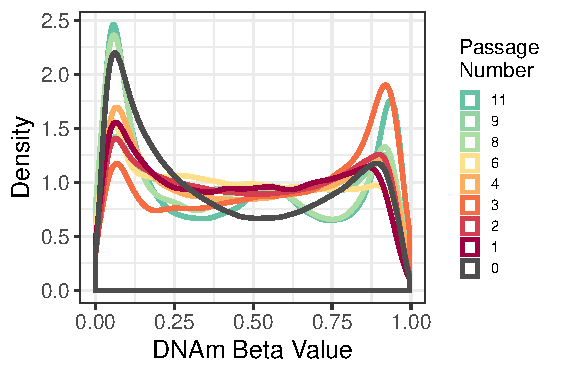
\includegraphics[width=1\textwidth]{../figs/MTAB4957_beta_notfetal_with_primary.pdf}}
\end{minipage}%
\hspace{5mm}
\begin{minipage}{.45\linewidth}
\centering
\sidesubfloat[]{\label{main:c}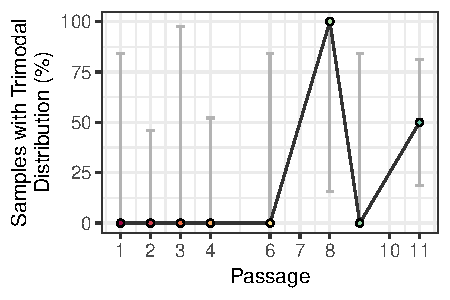
\includegraphics[width=1\textwidth]{../figs/MTAB4957_mixture_model_prior_I_threshold.pdf}}
\end{minipage}\par\bigskip

\flushleft
\sidesubfloat[]{\label{main:b}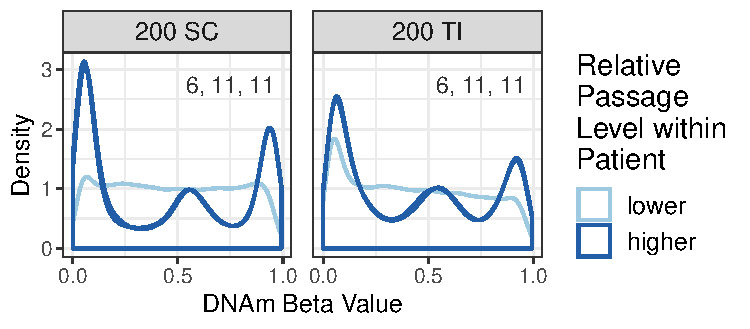
\includegraphics[width=0.5\textwidth]{../figs/MTAB4957_beta_paired_notfetal.pdf}}

\begin{minipage}{.45\linewidth}
\sidesubfloat[]{\label{main:a}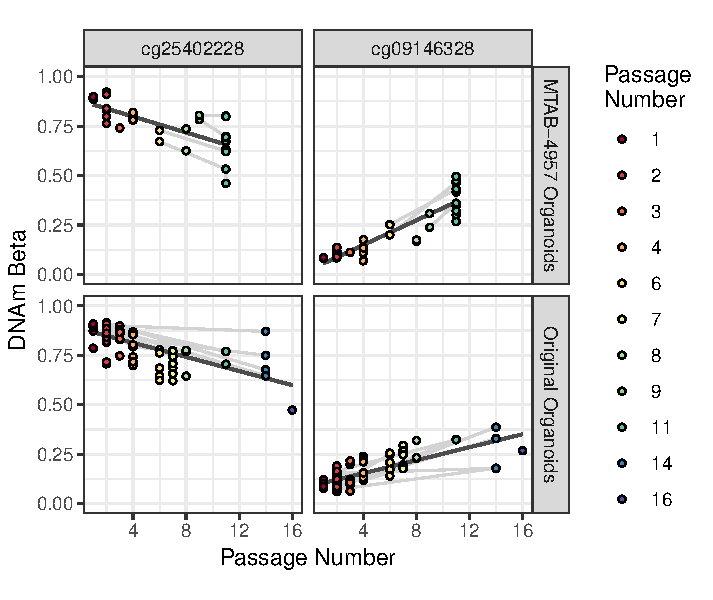
\includegraphics[width=1\textwidth]{../figs/Passage_differential_CpGs_MTAB4957.pdf}}
\end{minipage}%
\hspace{5mm}
\begin{minipage}{.45\linewidth}
\centering
\sidesubfloat[]{\label{main:c}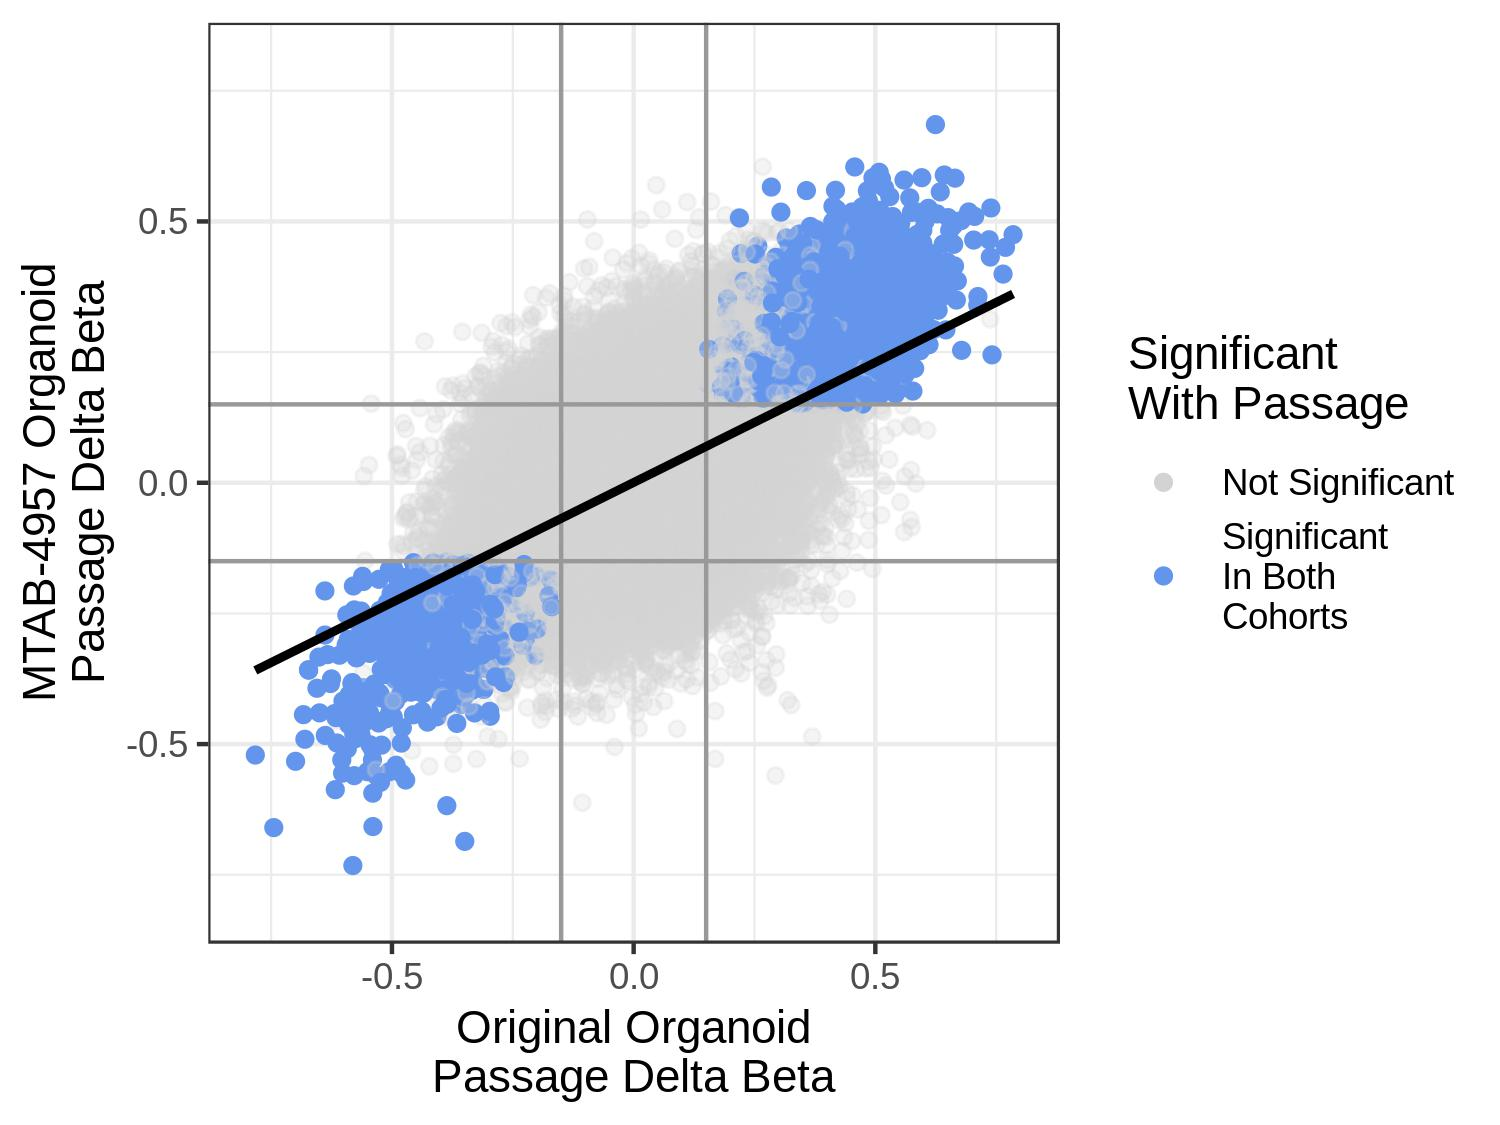
\includegraphics[width=1\textwidth]{../figs/jpeg/MTAB_db_directionality.jpeg}}
\end{minipage}\par\bigskip



\caption{\textbf{In E-MTAB-4957 pediatric organoids the DNAm beta value distribution for high passage samples is trimodial while for low passage samples it is bimodial.} All beta distributions displayed are for the 47,924 most variable CpGs. (a) Beta value distributions for all samples at a given passage number. Curves are coloured by the passage number. Included is the distribution for primary samples for comparison where passage is labelled as 0. (b) The percent of samples considered trimodal. Points are coloured by passage and the bars around each point represent the confidence interval for that percent. (c) Beta value distributions for samples derived from the same patient but cultured to a different number of passages. Plots are labelled with the patient ID number, sampling site of origin and the passage number of each sample derived from that patient and sampling site. Curves are coloured by high or low passage relative to the other sample(s).}
\label{fig:main}
\end{flushleft}
\end{figure}


\begin{figure}
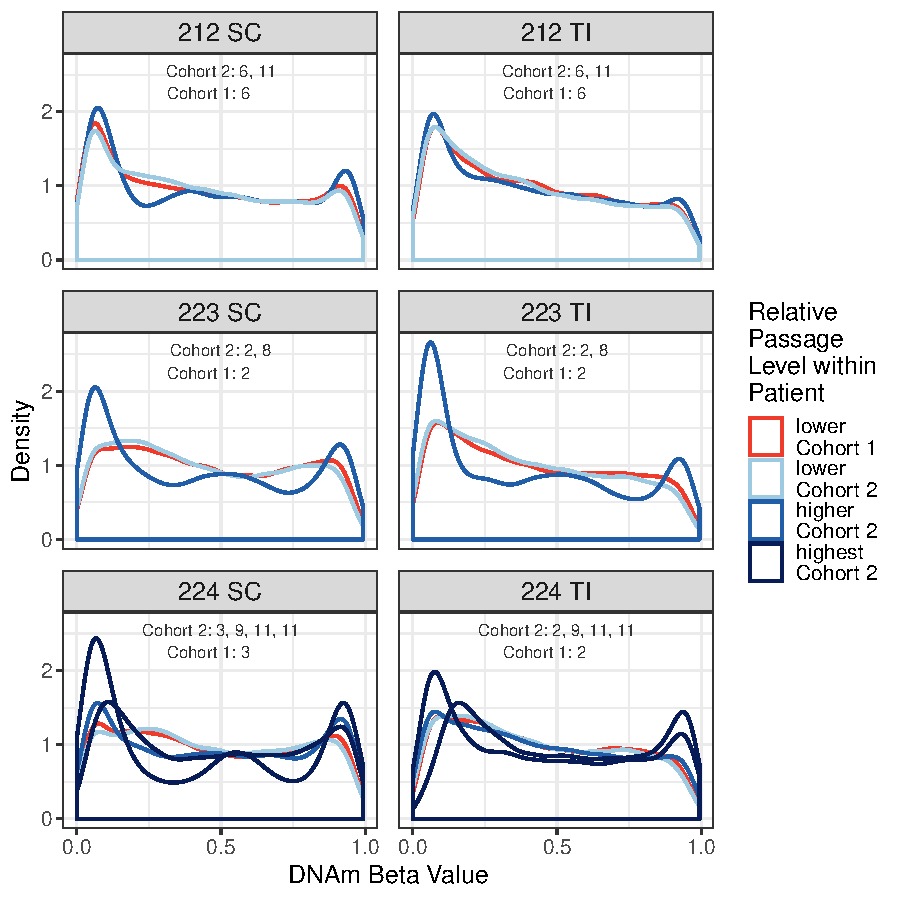
\includegraphics[width=1\textwidth]{../figs/MTAB4957_EPIC_beta_paired.pdf}
\caption{\textbf{In E-MTAB-4957 pediatric organoids the DNAm beta value distribution for high passage samples is trimodial while for low passage samples it is bimodial.} Beta value distributions for samples derived from the same patient but cultured to a different number of passages. Samples are shown which here if an individual's samples were run in both our organoids and E-MTAB-4957. All beta distributions displayed are for the 19,452 variable CpGs on both the 450K and EPIC. Plots are labelled with the patient ID number, sampling site of origin and the passage number of each sample derived from that patient and sampling site split by study. Curves are coloured by high or low passage relative to the other sample(s) and samples from our 165 organoid cohort are in red.}
\end{figure}




\begin{figure}
\begin{flushleft}

\begin{minipage}{.4\linewidth}
\sidesubfloat[]{\label{main:a}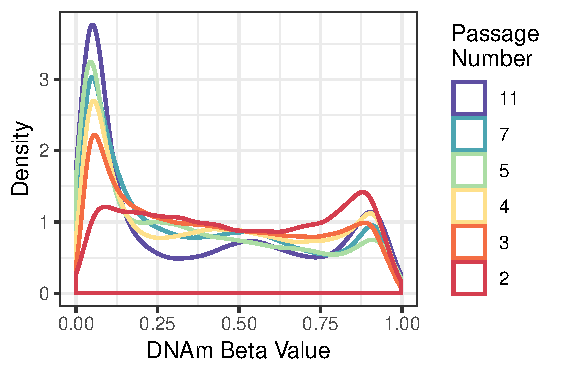
\includegraphics[width=1\textwidth]{../figs/GSE141256_variable_CpGs.pdf}}
\end{minipage}%
\hspace{5mm}
\begin{minipage}{.4\linewidth}
\centering
\sidesubfloat[]{\label{main:c}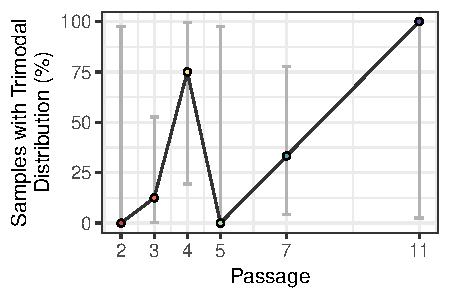
\includegraphics[width=1\textwidth]{../figs/GSE141256_Mixture_model_prior_I_threshold.pdf}}
\end{minipage}\par\bigskip

\flushleft
\sidesubfloat[]{\label{main:b}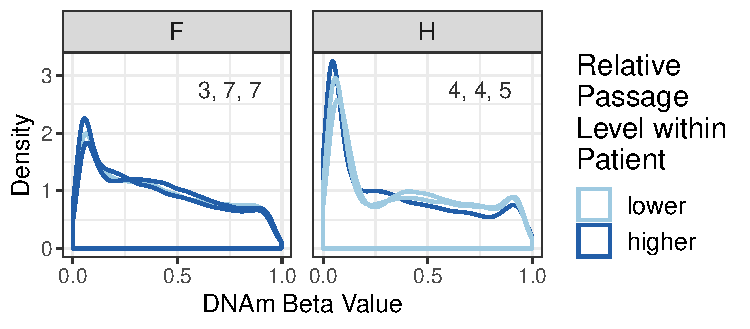
\includegraphics[width=0.5\textwidth]{../figs/GSE141256_paired_beta.pdf}}

\begin{minipage}{.45\linewidth}
\sidesubfloat[]{\label{main:a}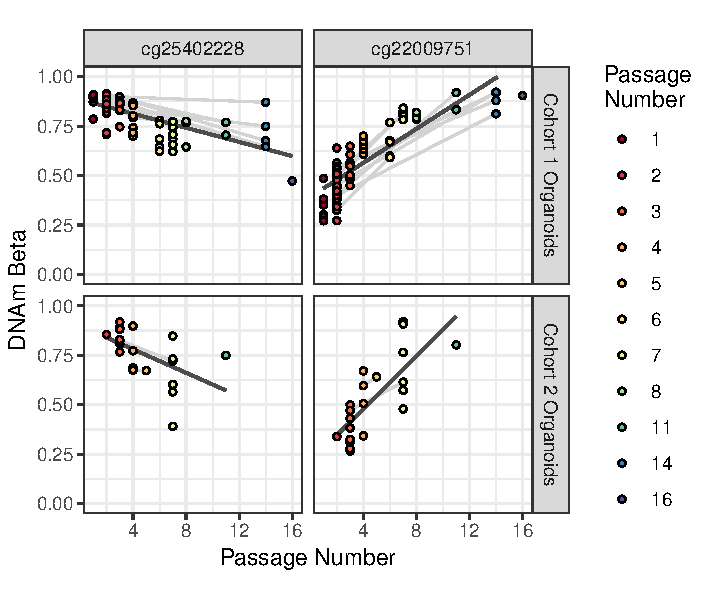
\includegraphics[width=1\textwidth]{../figs/Passage_differential_CpGs_GSE141256.pdf}}
\end{minipage}%
\hspace{5mm}
\begin{minipage}{.45\linewidth}
\centering
\sidesubfloat[]{\label{main:c}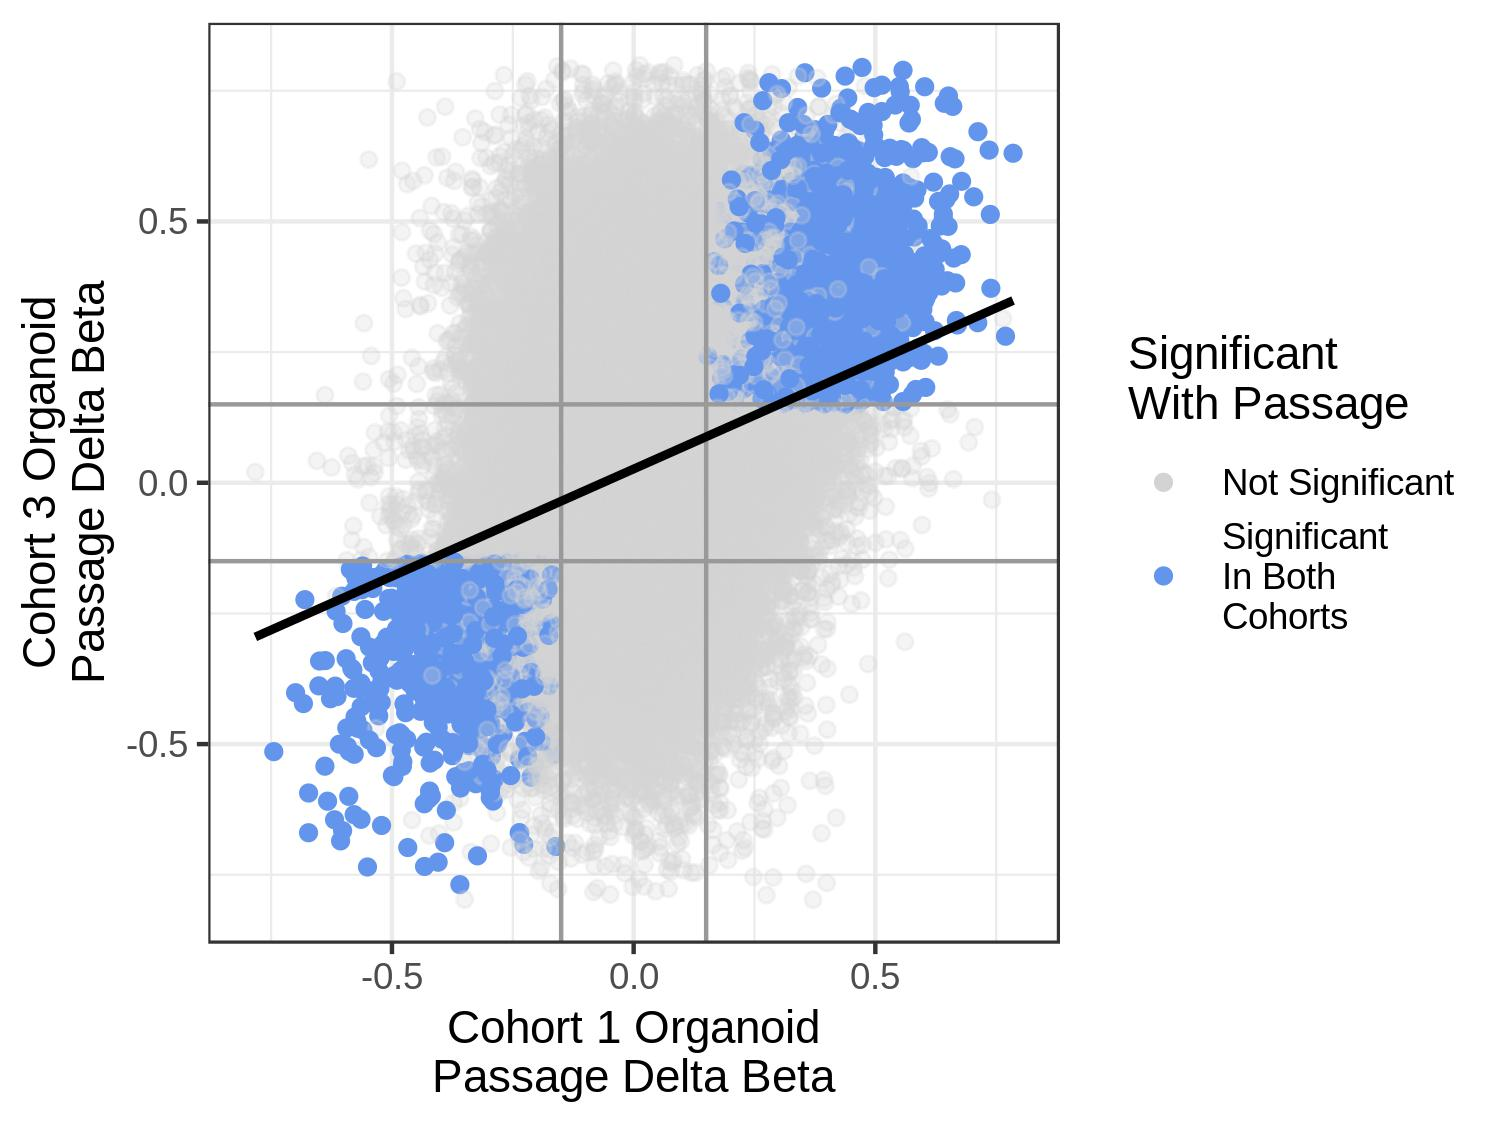
\includegraphics[width=1\textwidth]{../figs/jpeg/GSE141256_db_directionality.jpeg}}
\end{minipage}\par\bigskip



\caption{\textbf{In GSE141256 organoids the DNAm beta value distribution for high passage samples is trimodial while for low passage samples it is bimodial.} All beta distributions displayed are for the 55,379 most variable CpGs in fetal organoids. (a) Beta value distributions for all samples at a given passage number. Curves are coloured by the passage number. (b) The percent of samples considered trimodal. Points are coloured by passage and the bars around each point represent the confidence interval for that percent. (c) Beta value distributions for samples derived from the same patient but cultured to a different number of passages. Plots are labelled with the patient ID and the passage number of each sample derived from that patient. Curves are coloured by high or low passage relative to the other sample(s).}
\label{fig:GSE141256}
\end{flushleft}
\end{figure}




\begin{figure}
\begin{flushleft}

\begin{minipage}{.4\linewidth}
\sidesubfloat[]{\label{main:a}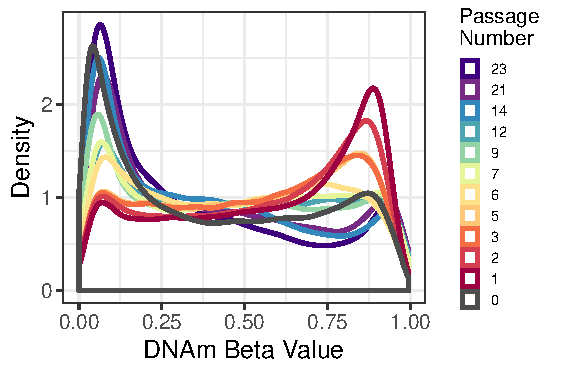
\includegraphics[width=1\textwidth]{../figs/MTAB4957_beta_fetal_with_primary.pdf}}
\end{minipage}%
\hspace{5mm}
\begin{minipage}{.4\linewidth}
\centering
\sidesubfloat[]{\label{main:c}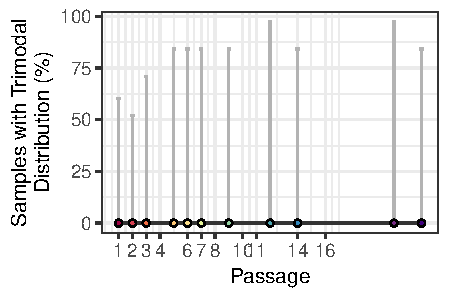
\includegraphics[width=1\textwidth]{../figs/MTAB4957_fetal_mixture_model_prior_I_threshold.pdf}}
\end{minipage}\par\bigskip

\centering
\sidesubfloat[]{\label{main:b}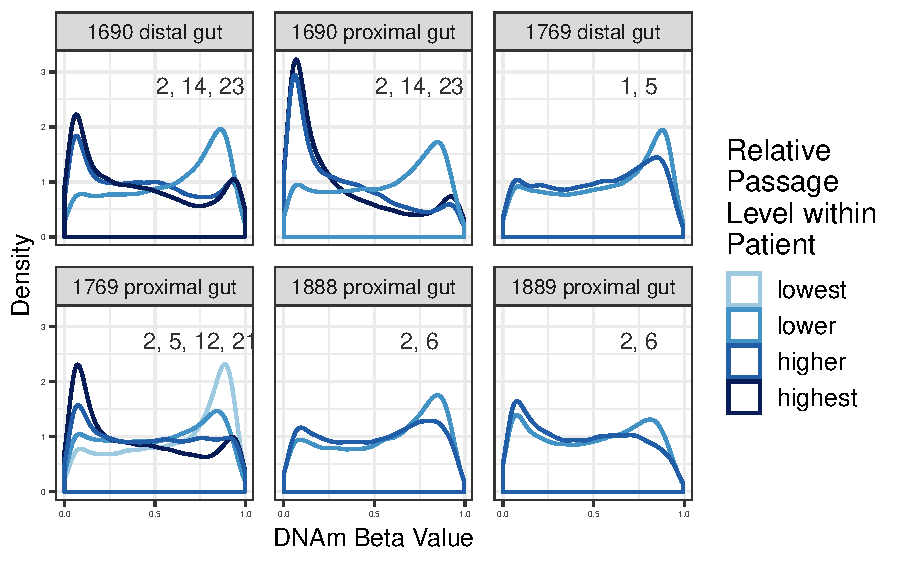
\includegraphics[width=0.8\textwidth]{../figs/MTAB4957_beta_paired_fetal.pdf}}

\begin{minipage}{.45\linewidth}
\sidesubfloat[]{\label{main:a}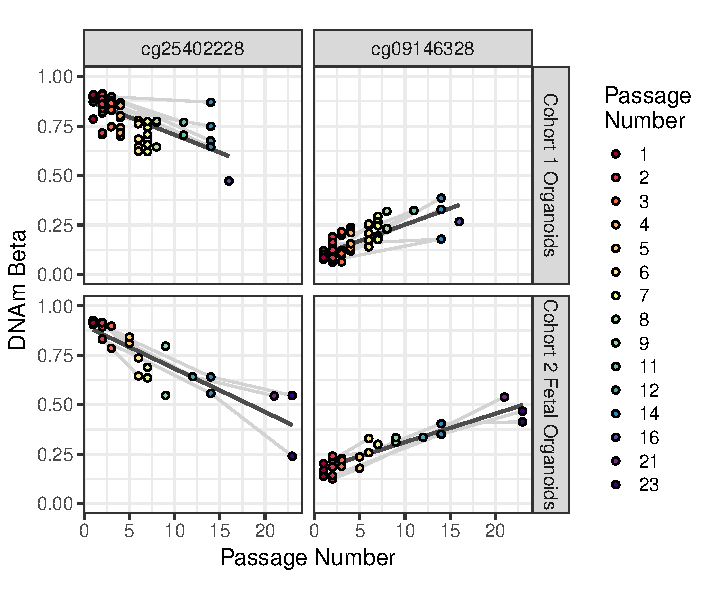
\includegraphics[width=1\textwidth]{../figs/Passage_differential_CpGs_MTAB4957_fetal.pdf}}
\end{minipage}%
\hspace{5mm}
\begin{minipage}{.45\linewidth}
\centering
\sidesubfloat[]{\label{main:c}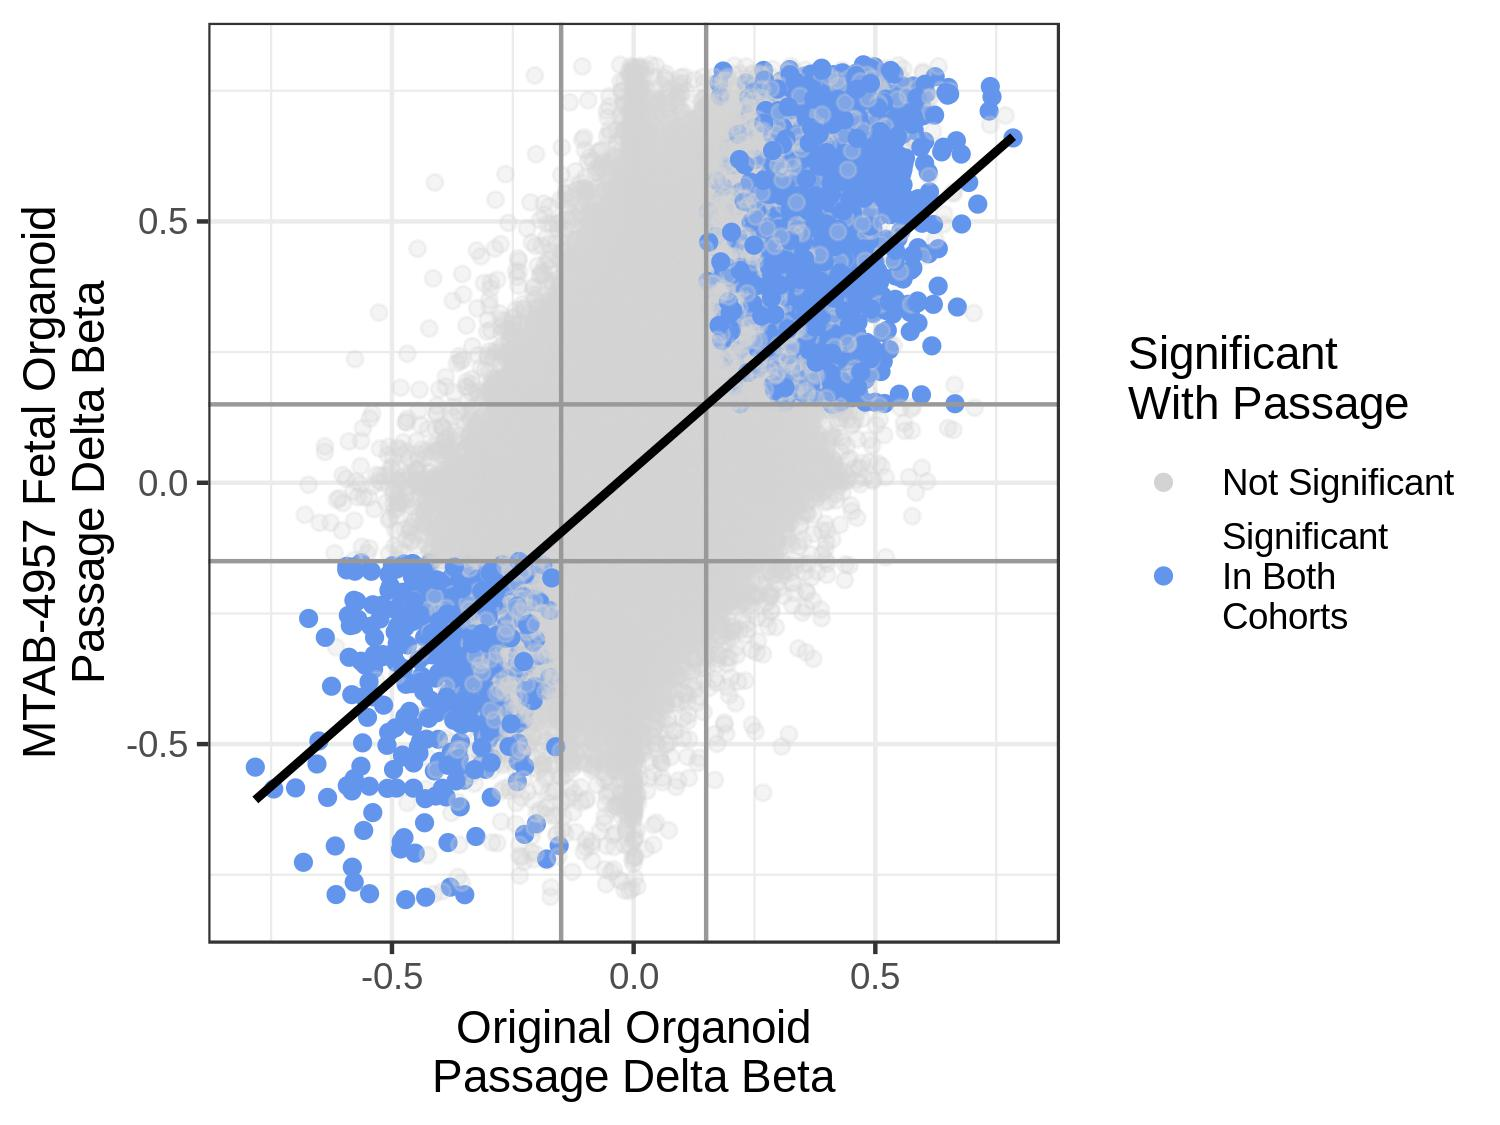
\includegraphics[width=1\textwidth]{../figs/jpeg/MTAB_db_directionality_fetal.jpeg}}
\end{minipage}\par\bigskip



\caption{\textbf{In E-MTAB-4957 fetal organoids the DNAm beta value distribution for high passage samples is more unmethylated than low passage samples.} All beta distributions displayed are for the 28,418 most variable CpGs in fetal organoids. (a) Beta value distributions for all samples at a given passage number. Curves are coloured by the passage number. Included is the distribution for primary samples for comparison where passage is labelled as 0. (b) The percent of samples considered trimodal. Points are coloured by passage and the bars around each point represent the confidence interval for that percent. (c) Beta value distributions for samples derived from the same patient but cultured to a different number of passages. Plots are labelled with the patient ID number, sampling site of origin and the passage number of each sample derived from that patient and sampling site. Curves are coloured by high or low passage relative to the other sample(s).}
\label{fig:fetal}
\end{flushleft}
\end{figure}






\begin{figure}
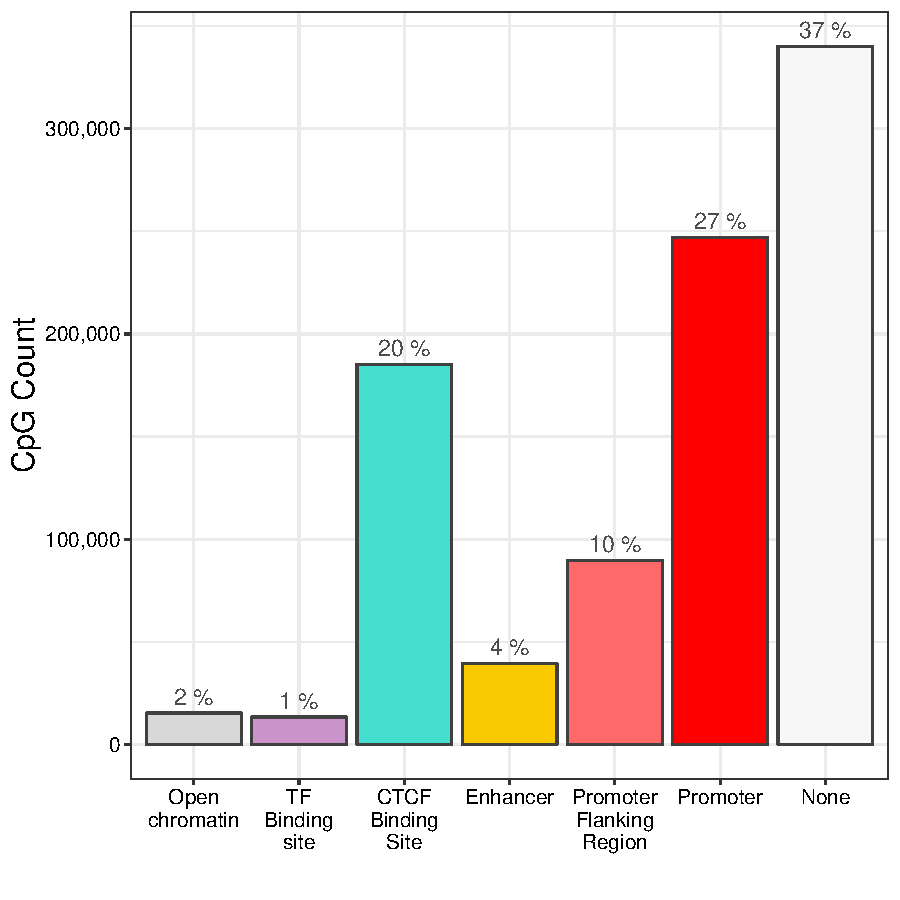
\includegraphics[width=0.8\textwidth]{../figs/EPIC_distribution_reg_CpGs.pdf}
\caption{\textbf{Background distribution of CpGs on the EPIC array.} Number of 800,383 EPIC array CpGs (used in this analysis) in regulatory genomic features.}
\end{figure}

\begin{figure}
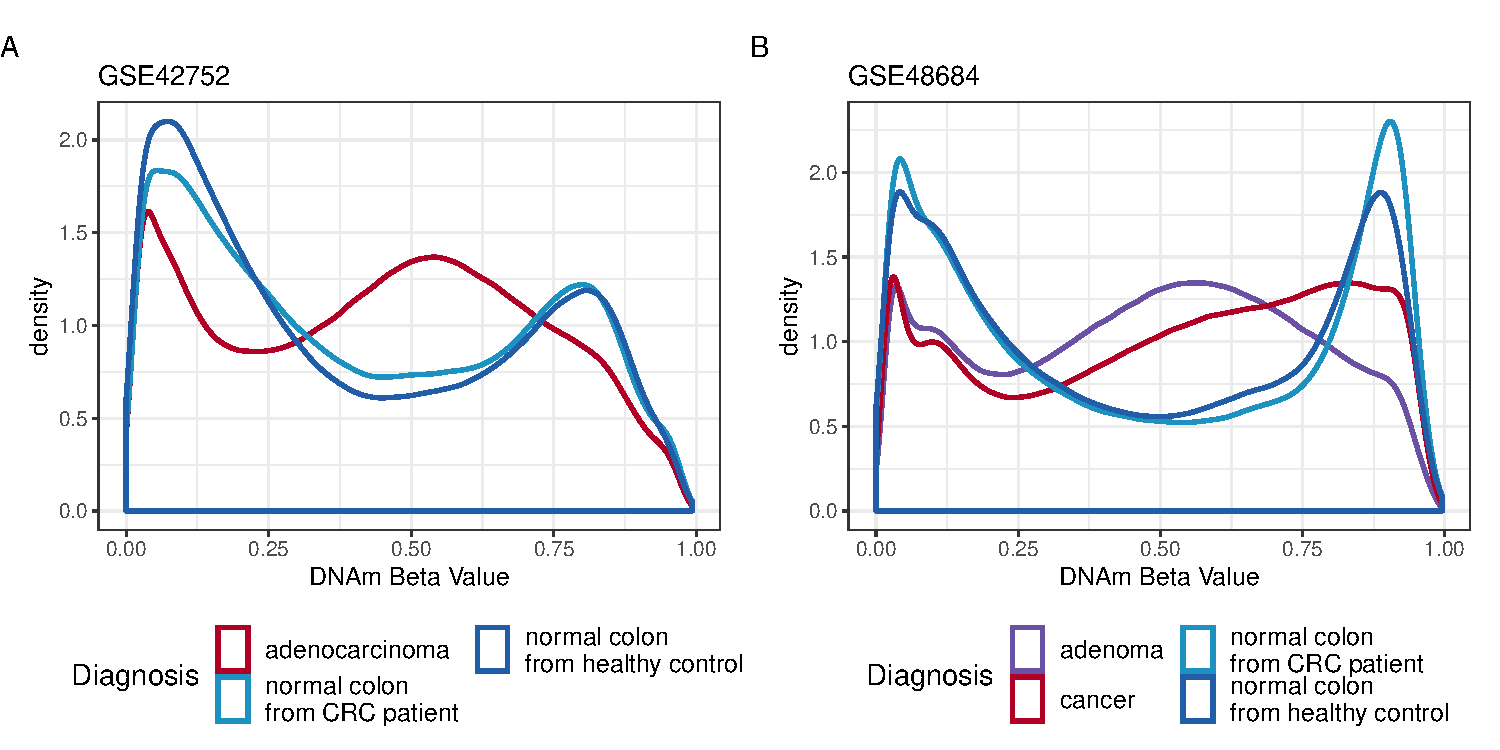
\includegraphics[width=1\textwidth]{../figs/cancer_public_same_variable_cpg_num.pdf}
\caption{\textbf{Appearance of the trimodal effect in three published cancer datasets.} In all datasets samples grouped by cancer diagnosis, curves show the DNAm distribution the top most variable CpGs. (a) GSE42752; 63 samples; colon samples (b) GSE48684; 147 samples; colon samples (c) GSE53051; 220 samples; For clarity plots are also split into tissue of origin. }
\end{figure}


\begin{figure}
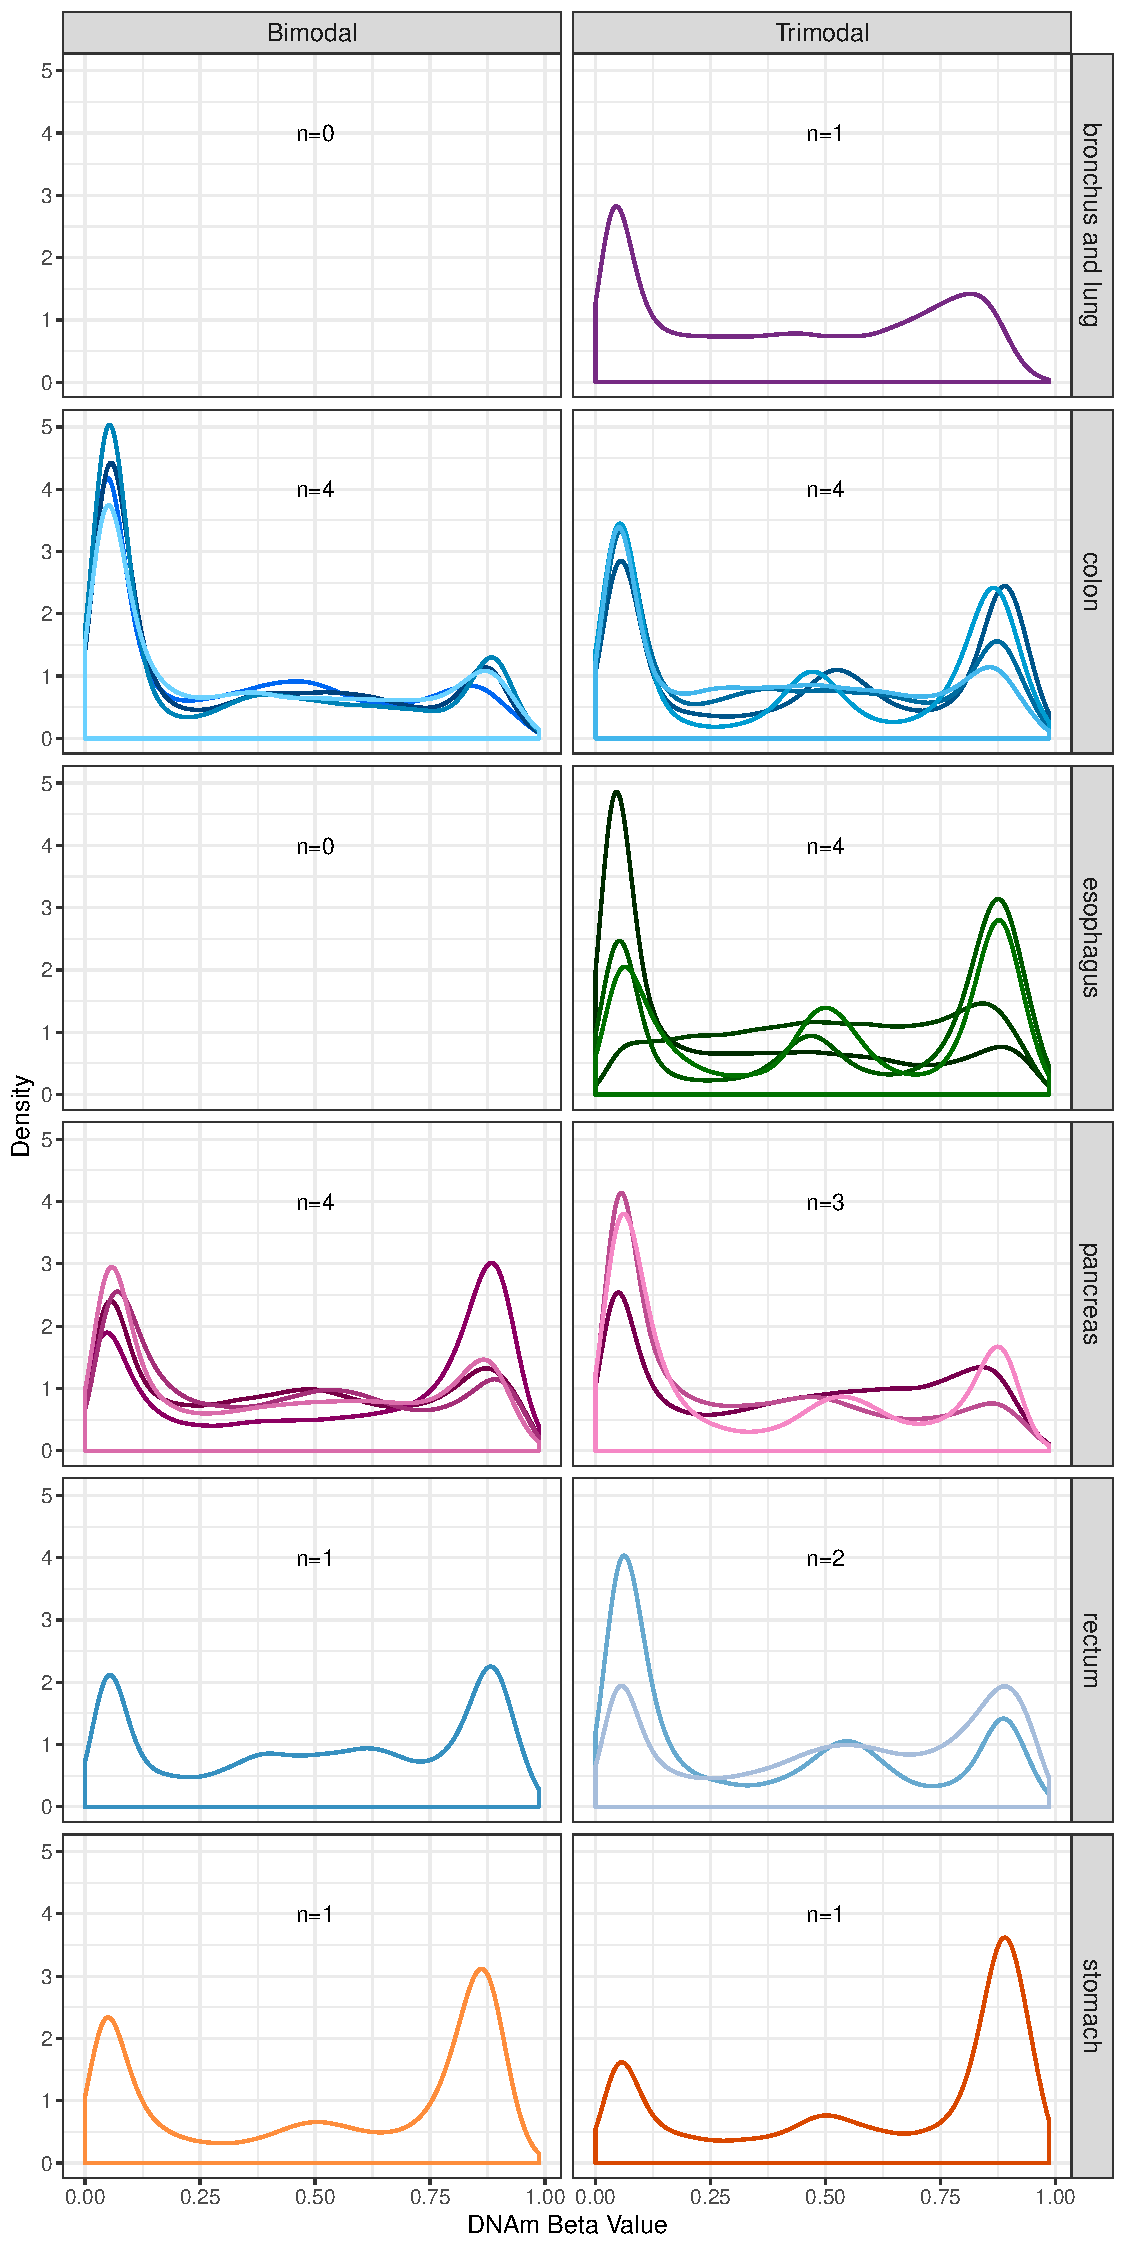
\includegraphics[width=0.7\textwidth]{../figs/GSE144213_variable_CpGs.pdf}
\caption{\textbf{Appearance of the trimodal effect in publicly available cancer organoid data (GSE142213).} Curves show the DNAm distribution the top 71,384 most variable CpGs. Samples are grouped by tissue of origin and separated by whether they are classified as tri or bimodal. }
\end{figure}





\end{document}